% !TeX program = xelatex
% 基于 YOLOv5s 的 PCB 表面缺陷检测与图像处理辅助分析 —— DocRescue 模板风格迁移候选版
% 编译: xelatex -> biber -> xelatex x2（参考文献迁移为 biblatex+gb7714-2015, 需用 biber 而非 bibtex）
\documentclass[UTF8,a4paper,zihao=5,twocolumn,fontset=fandol]{ctexart}

\usepackage[top=1.65cm,bottom=1.75cm,left=1.75cm,right=1.75cm]{geometry}
\usepackage{graphicx}
\usepackage[font=small,labelfont=bf,labelsep=quad]{caption}
\usepackage{booktabs}
\usepackage{amsmath}
\usepackage{float}
\usepackage{xcolor}
\usepackage{hyperref}
\usepackage[backend=biber,style=gb7714-2015,sorting=none]{biblatex}
\addbibresource{references.bib}

\graphicspath{{figures/}}

\setlength{\columnsep}{0.65cm}
\setlength{\parindent}{2em}
\setlength{\parskip}{0pt}
\setlength{\emergencystretch}{2em}
\renewcommand{\arraystretch}{1.08}
\raggedbottom

% DocRescue 模板: 放宽浮动体放置约束, 避免图表独占整页产生大面积空白
\renewcommand{\topfraction}{0.88}
\renewcommand{\bottomfraction}{0.55}
\renewcommand{\dbltopfraction}{0.92}
\renewcommand{\textfraction}{0.05}
\renewcommand{\floatpagefraction}{0.72}
\renewcommand{\dblfloatpagefraction}{0.72}
\setcounter{topnumber}{4}
\setcounter{dbltopnumber}{4}
\setcounter{totalnumber}{8}

\makeatletter
\setlength{\@fptop}{0pt}
\setlength{\@fpsep}{8pt plus 1fil}
\setlength{\@fpbot}{0pt plus 1fil}
\setlength{\@dblfptop}{0pt}
\setlength{\@dblfpsep}{8pt plus 1fil}
\setlength{\@dblfpbot}{0pt plus 1fil}
\makeatother

% DocRescue 模板: 链接与标题配色
\definecolor{ReportBlue}{HTML}{1F5A94}
\definecolor{ReportGray}{HTML}{4B5563}
\hypersetup{
  colorlinks=true,
  linkcolor=ReportBlue,
  citecolor=ReportBlue,
  urlcolor=ReportBlue,
  pdftitle={基于 YOLOv5s 的 PCB 表面缺陷检测与图像处理辅助分析}
}
\urlstyle{same}

% DocRescue 模板: 节标题格式
\ctexset{
  section={format=\large\bfseries\color{ReportBlue}},
  subsection={format=\normalsize\bfseries},
  subsubsection={format=\normalsize\bfseries\color{ReportGray}}
}
\AtBeginBibliography{\small}

% DocRescue 模板: \maketitle 标题区(内容仍为本项目信息)
\title{\bfseries 基于 YOLOv5s 的 PCB 表面缺陷检测与图像处理辅助分析\\
\large 数字图像处理课程大作业报告}
\author{覃天祥\quad 23339096\\
\small 中山大学数学学院（珠海）\\
\small 课程：数字图像处理\quad 任课教师：邝东阳}
\date{2026 年 7 月}

\begin{document}

\maketitle

\begin{abstract}
本文基于公开 DeepPCB 数据集完成 PCB 表面缺陷检测课程项目。项目首先将
DeepPCB 标注转换为 YOLO 格式，并训练 YOLOv5s 完成 open、short、mousebite、spur、copper、
pin\_hole 六类缺陷检测；同时利用模板图与待测图已配准的特点，实现了基于模板差分、Otsu 阈值、
形态学处理和连通域分析的类别无关缺陷候选方法，用于体现数字图像处理方法在该任务中的作用。
在官方测试集上，YOLOv5s 取得 Precision 0.951、Recall 0.944、mAP50 0.968、mAP50:95 0.594；
传统图像处理方法在 IoU$=$0.33 下取得 F1 0.658。实验结果表明，深度检测模型在六类缺陷识别上
表现较好，而传统差分方法能够提供直观的候选区域和错误分析依据。
\end{abstract}

\noindent\textbf{关键词：}PCB 缺陷检测；YOLOv5s；DeepPCB；模板差分；Otsu 阈值；形态学处理；连通域分析

\section{引言}

印刷电路板（PCB）制造过程中的断路（open）、短路（short）、鼠咬（mousebite）、毛刺（spur）、
余铜（spurious copper）与针孔（pin-hole）等表面缺陷会直接影响电路功能，自动化的缺陷检测因此是
工业视觉的经典问题之一。近年来以 YOLO~\cite{redmon2016yolo} 系列为代表的深度目标检测方法在
该类任务上表现出色；与此同时，PCB 检测场景往往具有一个传统方法可以直接利用的先验——
待测板图像可以与无缺陷的模板图像配准对齐，通过差分即可暴露外观差异，这恰好对应数字图像处理课程中
灰度变换、图像差分、阈值分割、形态学处理与连通域分析等核心内容~\cite{gonzalez2018dip}。

本文选取公开数据集 DeepPCB~\cite{tang2019deeppcb}，完成三部分工作：
（1）对官方数据进行核查与 YOLO 格式转换，并以脚本化自检保证转换正确；
（2）以官方预训练权重为起点训练 YOLOv5s~\cite{jocher2020yolov5} 六类缺陷检测模型，
在官方测试集上报告结果；
（3）实现一个"模板差分 + Otsu + 形态学 + 连通域"的传统图像处理候选区域生成模块，
在与检测主线一致的数据划分下给出框级定量结果，并进行错误分析与互补性讨论。
需要说明的是，本文定位为课程大作业的完整实践与分析，不声称方法创新；传统模块是类别无关
的缺陷候选基线方法，不是六类分类器。

\section{数据集与标注转换}

\subsection{DeepPCB 概况与实测核查}

DeepPCB 包含 1500 组图像对，每组由一张无缺陷模板图（\verb|*_temp.jpg|）与一张经配准对齐的
待测图（\verb|*_test.jpg|）组成，图像来自线阵 CCD 扫描并经二值化预处理。我们对全部文件做了
脚本化核查：1500 张待测图实测均为 $640\times640$（其中 1462 张灰度、38 张 RGB），
标注文件共 10013 行且无一异常（无越界坐标、无非法类别）。一个与官方 README 不一致的实测发现：
README 描述标注为逗号分隔 \verb|x1,y1,x2,y2,type|，而全部 10013 行实际为\textbf{空格分隔}，
转换脚本据此按空格解析。缺陷框宽度范围 18--173\,px（均值 38.9），高度 19--152\,px（均值 35.7），
属中小目标；每图 1--15 个缺陷（均值 6.68）。

\subsection{格式转换与数据划分}

标注转换按下式将像素坐标框转为 YOLO 归一化格式（逐图读取实际宽高 $W,H$，不假设 640）：
\begin{equation}
\begin{aligned}
x_c &= \tfrac{(x_1+x_2)/2}{W}, & y_c &= \tfrac{(y_1+y_2)/2}{H},\\
w &= \tfrac{x_2-x_1}{W}, & h &= \tfrac{y_2-y_1}{H},
\end{aligned}
\end{equation}
类别映射为 class\_id $=$ type $-1$，即 open$=$0、short$=$1、mousebite$=$2、spur$=$3、
copper$=$4、pin\_hole$=$5（copper 在报告中可解释为 spurious copper，代码与配置统一写 copper）。
划分沿用官方协议：对 YOLOv5s 检测主线，官方 test.txt 的 500 张仅在模型训练完成、
权重固定后用于最终评估（传统图像处理模块的外扩边距设置见 3.2 节与第 6 节）；
官方 trainval.txt 的 1000 张
以固定随机种子 20260712、按 board group 内最大余数法配额抽样，划分为 train 900 / val 100。
表~\ref{tab:split} 与表~\ref{tab:classmap} 给出统计，图~\ref{fig:classdist} 与
图~\ref{fig:bboxwh} 给出类别分布与框尺寸分布。

值得注意的是官方划分的 group 构成：test 的 500 张中有 332 张（66.4\%）来自 train/val 中
从未出现过的 4 个 board group（12000、12100、12300、90100）。因此 test 结果在一定程度上
包含了对\textbf{未见 group}的适应，但这只是 group 级的板面差异，不应引申为对工业场景的泛化能力。

\begin{figure}[t]
  \centering
  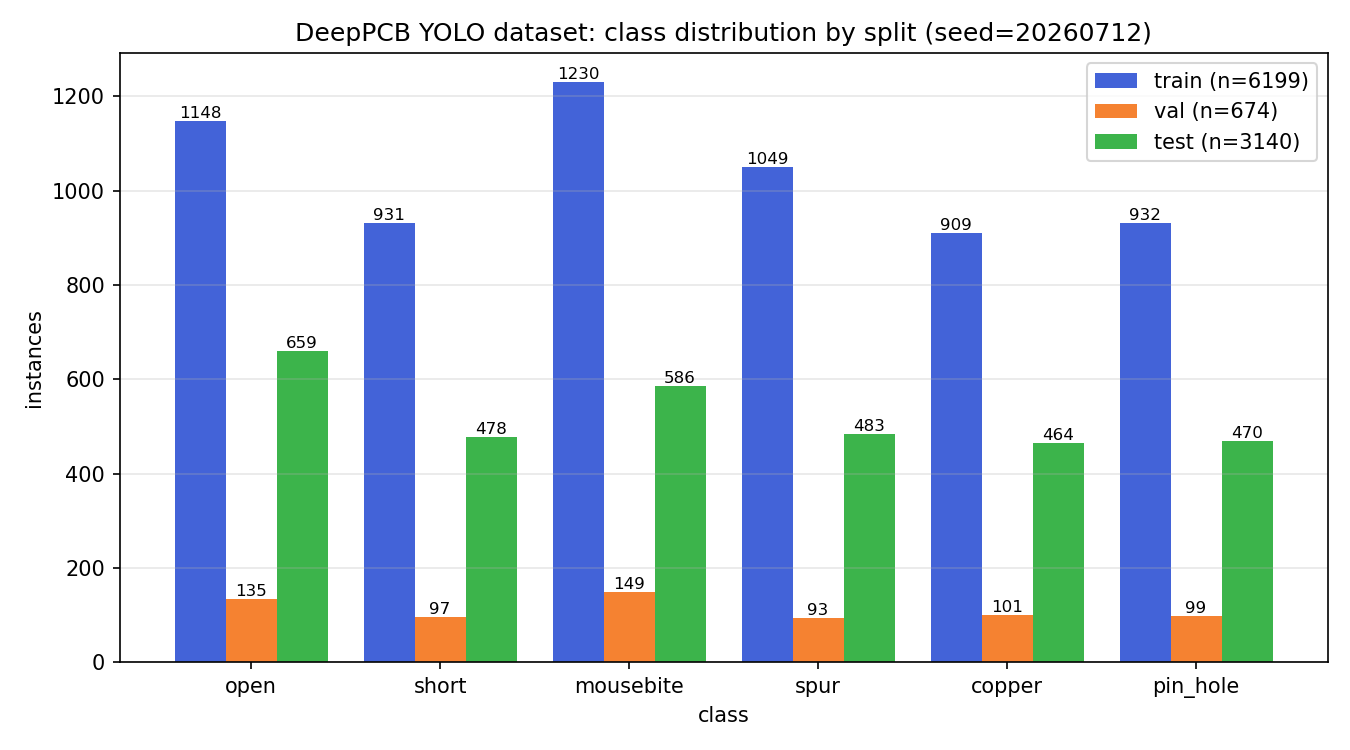
\includegraphics[width=\columnwidth]{class_distribution.png}
  \caption{六类缺陷在 train/val/test 上的实例分布（转换后 YOLO 标签实测统计）。}
  \label{fig:classdist}
\end{figure}

\begin{figure}[t]
  \centering
  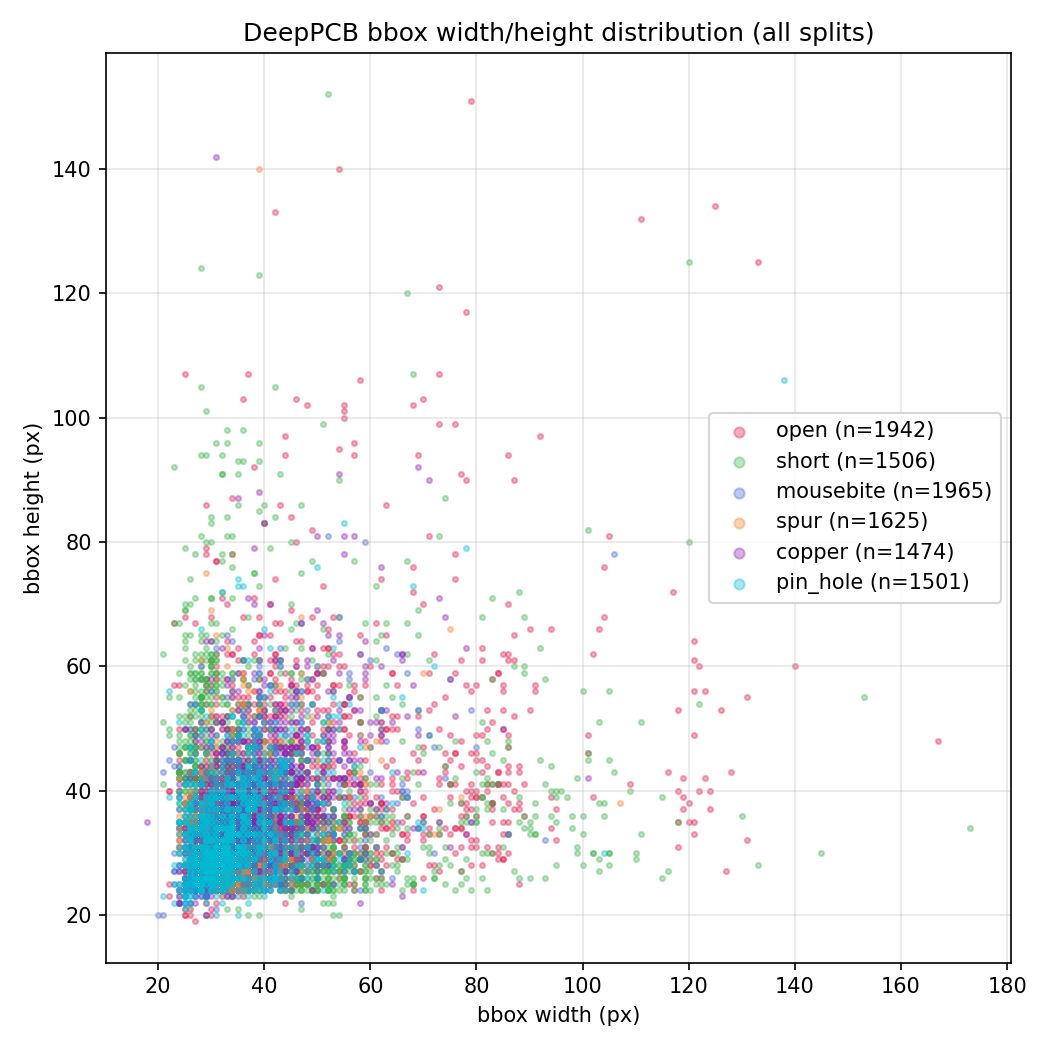
\includegraphics[width=0.92\columnwidth]{bbox_wh_distribution.png}
  \caption{全部 10013 个缺陷框的宽高分布（像素，按类别着色）。}
  \label{fig:bboxwh}
\end{figure}

\begin{table}[t]
\centering
\caption{数据划分（划分种子 20260712；train/val 按 group 内最大余数法配额从官方 trainval 划出，test 为官方测试集）}
\label{tab:split}
\small
\begin{tabular}{lccc}
\toprule
划分 & 图像数 & 缺陷框数 & 每图平均框数 \\
\midrule
train & 900 & 6199 & 6.89 \\
val & 100 & 674 & 6.74 \\
test & 500 & 3140 & 6.28 \\
\midrule
合计 & 1500 & 10013 & 6.68 \\
\bottomrule
\end{tabular}
\end{table}

\begin{table}[t]
\centering
\caption{类别映射与各划分实例数（源标注 type $1\!-\!6$ 映射为 YOLO class\_id $=$ type $-1$；copper 即 spurious copper，余铜）}
\label{tab:classmap}
\small
\setlength{\tabcolsep}{3pt}
\begin{tabular}{clcccc}
\toprule
id & 类别 & train & val & test & 合计 \\
\midrule
0 & open（断路） & 1148 & 135 & 659 & 1942 \\
1 & short（短路） & 931 & 97 & 478 & 1506 \\
2 & mousebite（鼠咬） & 1230 & 149 & 586 & 1965 \\
3 & spur（毛刺） & 1049 & 93 & 483 & 1625 \\
4 & copper（余铜） & 909 & 101 & 464 & 1474 \\
5 & pin\_hole（针孔） & 932 & 99 & 470 & 1501 \\
\midrule
 & 合计 & 6199 & 674 & 3140 & 10013 \\
\bottomrule
\end{tabular}
\end{table}


\subsection{转换自检}

通过自动化脚本检查了标签合法性、数据划分一致性和逐图框数，训练、评估和传统模块运行后
复查结果保持一致。此外将转换后标签反绘回图像做人工抽查（30 张，覆盖三个划分与六类），
框位置与缺陷语义一致。

\section{方法}

\subsection{YOLOv5s 六类缺陷检测}

YOLOv5s 是单阶段锚框检测器，采用 CSP 结构骨干与 PAN 特征融合，在 P3--P5 三个尺度上预测。
本文使用官方仓库 master 代码与 COCO 预训练权重 yolov5s.pt，仅将输出类别数改为 6
（由数据配置自动完成），未修改网络结构。模型参数量约 7.0M、计算量 16.0 GFLOPs。
训练前的 AutoAnchor 检查显示默认锚框对本数据集的 Best Possible Recall 为 1.000
（6.14 anchors/target），无需重新聚类，这与图~\ref{fig:bboxwh} 所示的中小目标分布一致。

\subsection{传统图像处理候选区域生成}

传统模块充分利用"模板--待测图已配准"的先验，流水线为：
（1）灰度化读取模板图与待测图；
（2）绝对差分 $D=|I_{\text{test}}-I_{\text{temp}}|$；
（3）$5\times5$ 中值滤波抑制配准残差产生的细边缘毛刺；
（4）Otsu 自动阈值~\cite{otsu1979threshold}逐图二值化；
（5）形态学开运算（$3\times3$ 椭圆核，去噪）与闭运算（$5\times5$ 椭圆核，连接断裂区域）
~\cite{gonzalez2018dip}；
（6）8 连通域分析得到候选区域；
（7）按面积（$\ge$50\,px$^2$）、最小宽高（$\ge$8\,px）与最大宽高（$\le$250\,px）过滤；
（8）候选框每侧外扩 PAD$=$10\,px 后裁剪到图像内。
候选得分定义为连通域内平均差分强度除以 255，用于匹配排序与结果输出。

外扩步骤（8）需要特别说明。DeepPCB 的真值框在缺陷像素之外带有明显的标注边距，
而连通域外接框紧贴缺陷像素。初步可视化检查发现，候选区域普遍落在缺陷附近，但两类框的
尺度约定不同，导致 IoU 难以达到匹配阈值（无外扩时 IoU$=$0.33 下 F1 仅 0.047）。
为对齐框尺寸约定，我们在 \textbf{val 划分}上扫描 PAD$\in\{0,4,\dots,16\}$ 并固定为 10\,px
（表~\ref{tab:pad_sweep}），随后才在测试集上运行；8--14\,px 为平台区，说明该值的选择稳健。
评价采用简单可核查的框级贪心匹配：候选按得分降序依次匹配 IoU 最大且未被占用的真值框，
每个真值框至多匹配一次；IoU 阈值取 0.33（DeepPCB 官方评估脚本的默认 IoU 约束，宽松定位参考）
与 0.50（常见检测阈值）两档。该模块为无类别候选生成，不输出缺陷类别。

\section{实验设置}

\textbf{环境。}Windows 11，NVIDIA GeForce RTX 5080 Laptop GPU（16\,GB），
Python 3.12.13，PyTorch 2.7.1+cu128，YOLOv5 官方 master（commit 2885cb4），
ultralytics 8.4.83。传统模块基于 OpenCV 4.11.0。

\textbf{训练。}输入 $640\times640$，batch size 16，SGD（lr$_0=0.01$，momentum 0.937，
weight decay $5\times10^{-4}$，warmup 3 epoch），采用官方 hyp.scratch-low 默认数据增强
（mosaic 1.0、水平翻转 0.5、HSV 扰动等），混合精度训练，共 50 epoch，
用时约 0.098 小时。训练随机种子为 train.py 默认值 0，与 2.2 节的数据划分种子
20260712 是两个相互独立的设置。正式训练前先以 2 epoch 短轮次预实验验证了数据管线与环境。
最优模型权重按 fitness（$0.1\cdot$mAP50 $+\,0.9\cdot$mAP50:95，在 val 上计算）选取，
best.pt 对应第 38 epoch；val 在本文中仅用于训练监控与最优权重选择。

\textbf{评估。}检测主线用官方 val.py 在官方测试集上评估（conf 0.001、NMS IoU 0.6），
报告 Precision、Recall、mAP50、mAP50:95。同一权重在官方测试集上复跑后，主要指标与首次评估一致。
传统模块按第 3.2 节协议评估。

\section{实验结果与分析}

\subsection{YOLOv5s 官方测试集结果}

表~\ref{tab:yolo_overall} 与表~\ref{tab:yolo_perclass} 给出总体与分类别结果：
总体 P 0.951、R 0.944、mAP50 0.968、mAP50:95 0.594，单图推理约 2\,ms（batch 16）。
六类 mAP50 均不低于 0.912；copper 的 mAP50:95 最高（0.734），
short 各项指标相对最弱（R 0.863、mAP50:95 0.482），
pin\_hole 呈"查全高、查准偏低"（R 0.979、P 0.865）。
作为参考，best.pt 在 val（100 图）上的最终验证为 P 0.978 / R 0.973 / mAP50 0.985 /
mAP50:95 0.651，test 相对 val 的回落可能与前述 66.4\% 未见 group 的构成有关，
提示官方测试集中存在一定 group 级分布差异（本文未做分 group 的检测指标统计，
此处仅为定性推测）。图~\ref{fig:pr} 与图~\ref{fig:cm} 给出 PR 曲线与混淆矩阵，
图~\ref{fig:pred} 为测试集预测拼图示例。

\begin{table}[t]
\centering
\caption{YOLOv5s 在官方 test 划分（500 图、3140 框）上的总体指标}
\label{tab:yolo_overall}
\small
\begin{tabular}{lcccc}
\toprule
划分 & Precision & Recall & mAP50 & mAP50:95 \\
\midrule
test & 0.951 & 0.944 & 0.968 & 0.594 \\
\bottomrule
\end{tabular}
\end{table}

\begin{table}[t]
\centering
\caption{YOLOv5s 官方 test 六类分项指标}
\label{tab:yolo_perclass}
\small
\setlength{\tabcolsep}{3.5pt}
\begin{tabular}{lccccc}
\toprule
类别 & 实例数 & P & R & mAP50 & mAP50:95 \\
\midrule
open & 659 & 0.973 & 0.973 & 0.976 & 0.547 \\
short & 478 & 0.936 & 0.863 & 0.912 & 0.482 \\
mousebite & 586 & 0.969 & 0.951 & 0.981 & 0.572 \\
spur & 483 & 0.985 & 0.927 & 0.970 & 0.606 \\
copper & 464 & 0.980 & 0.970 & 0.982 & 0.734 \\
pin\_hole & 470 & 0.865 & 0.979 & 0.986 & 0.623 \\
\bottomrule
\end{tabular}
\end{table}


\begin{figure}[t]
  \centering
  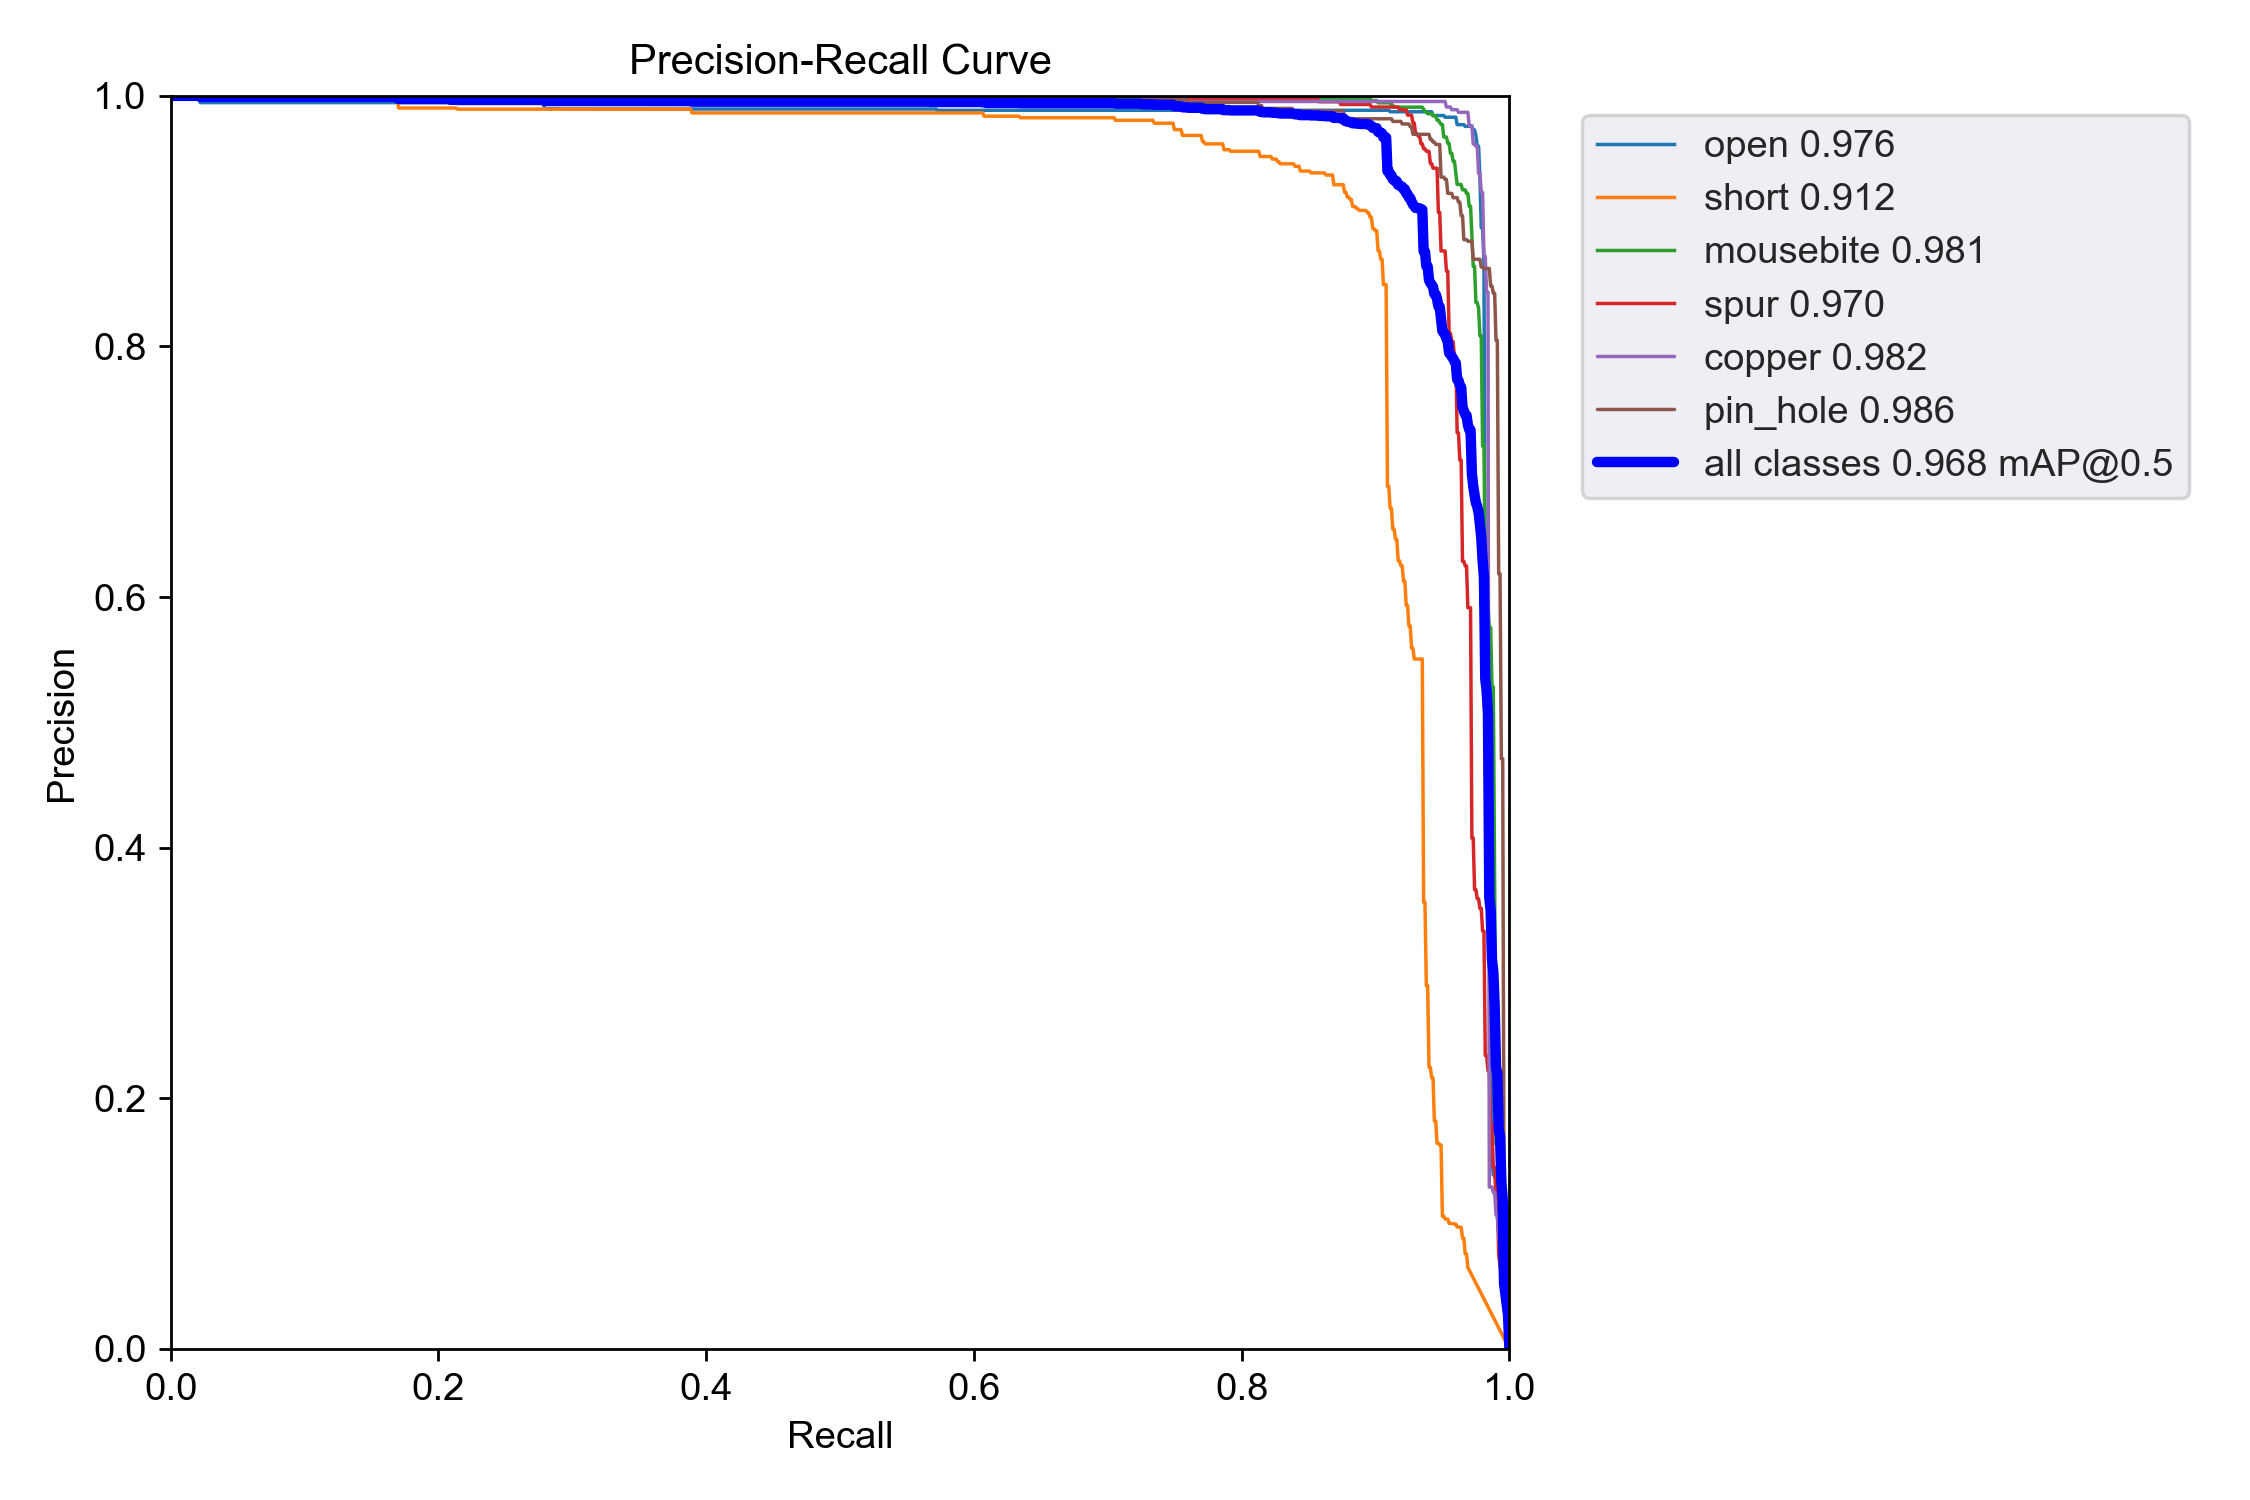
\includegraphics[width=0.94\columnwidth]{yolo_test_PR_curve.png}
  \caption{YOLOv5s 在官方测试集上的 PR 曲线（mAP@0.5）。}
  \label{fig:pr}
\end{figure}

\begin{figure}[t]
  \centering
  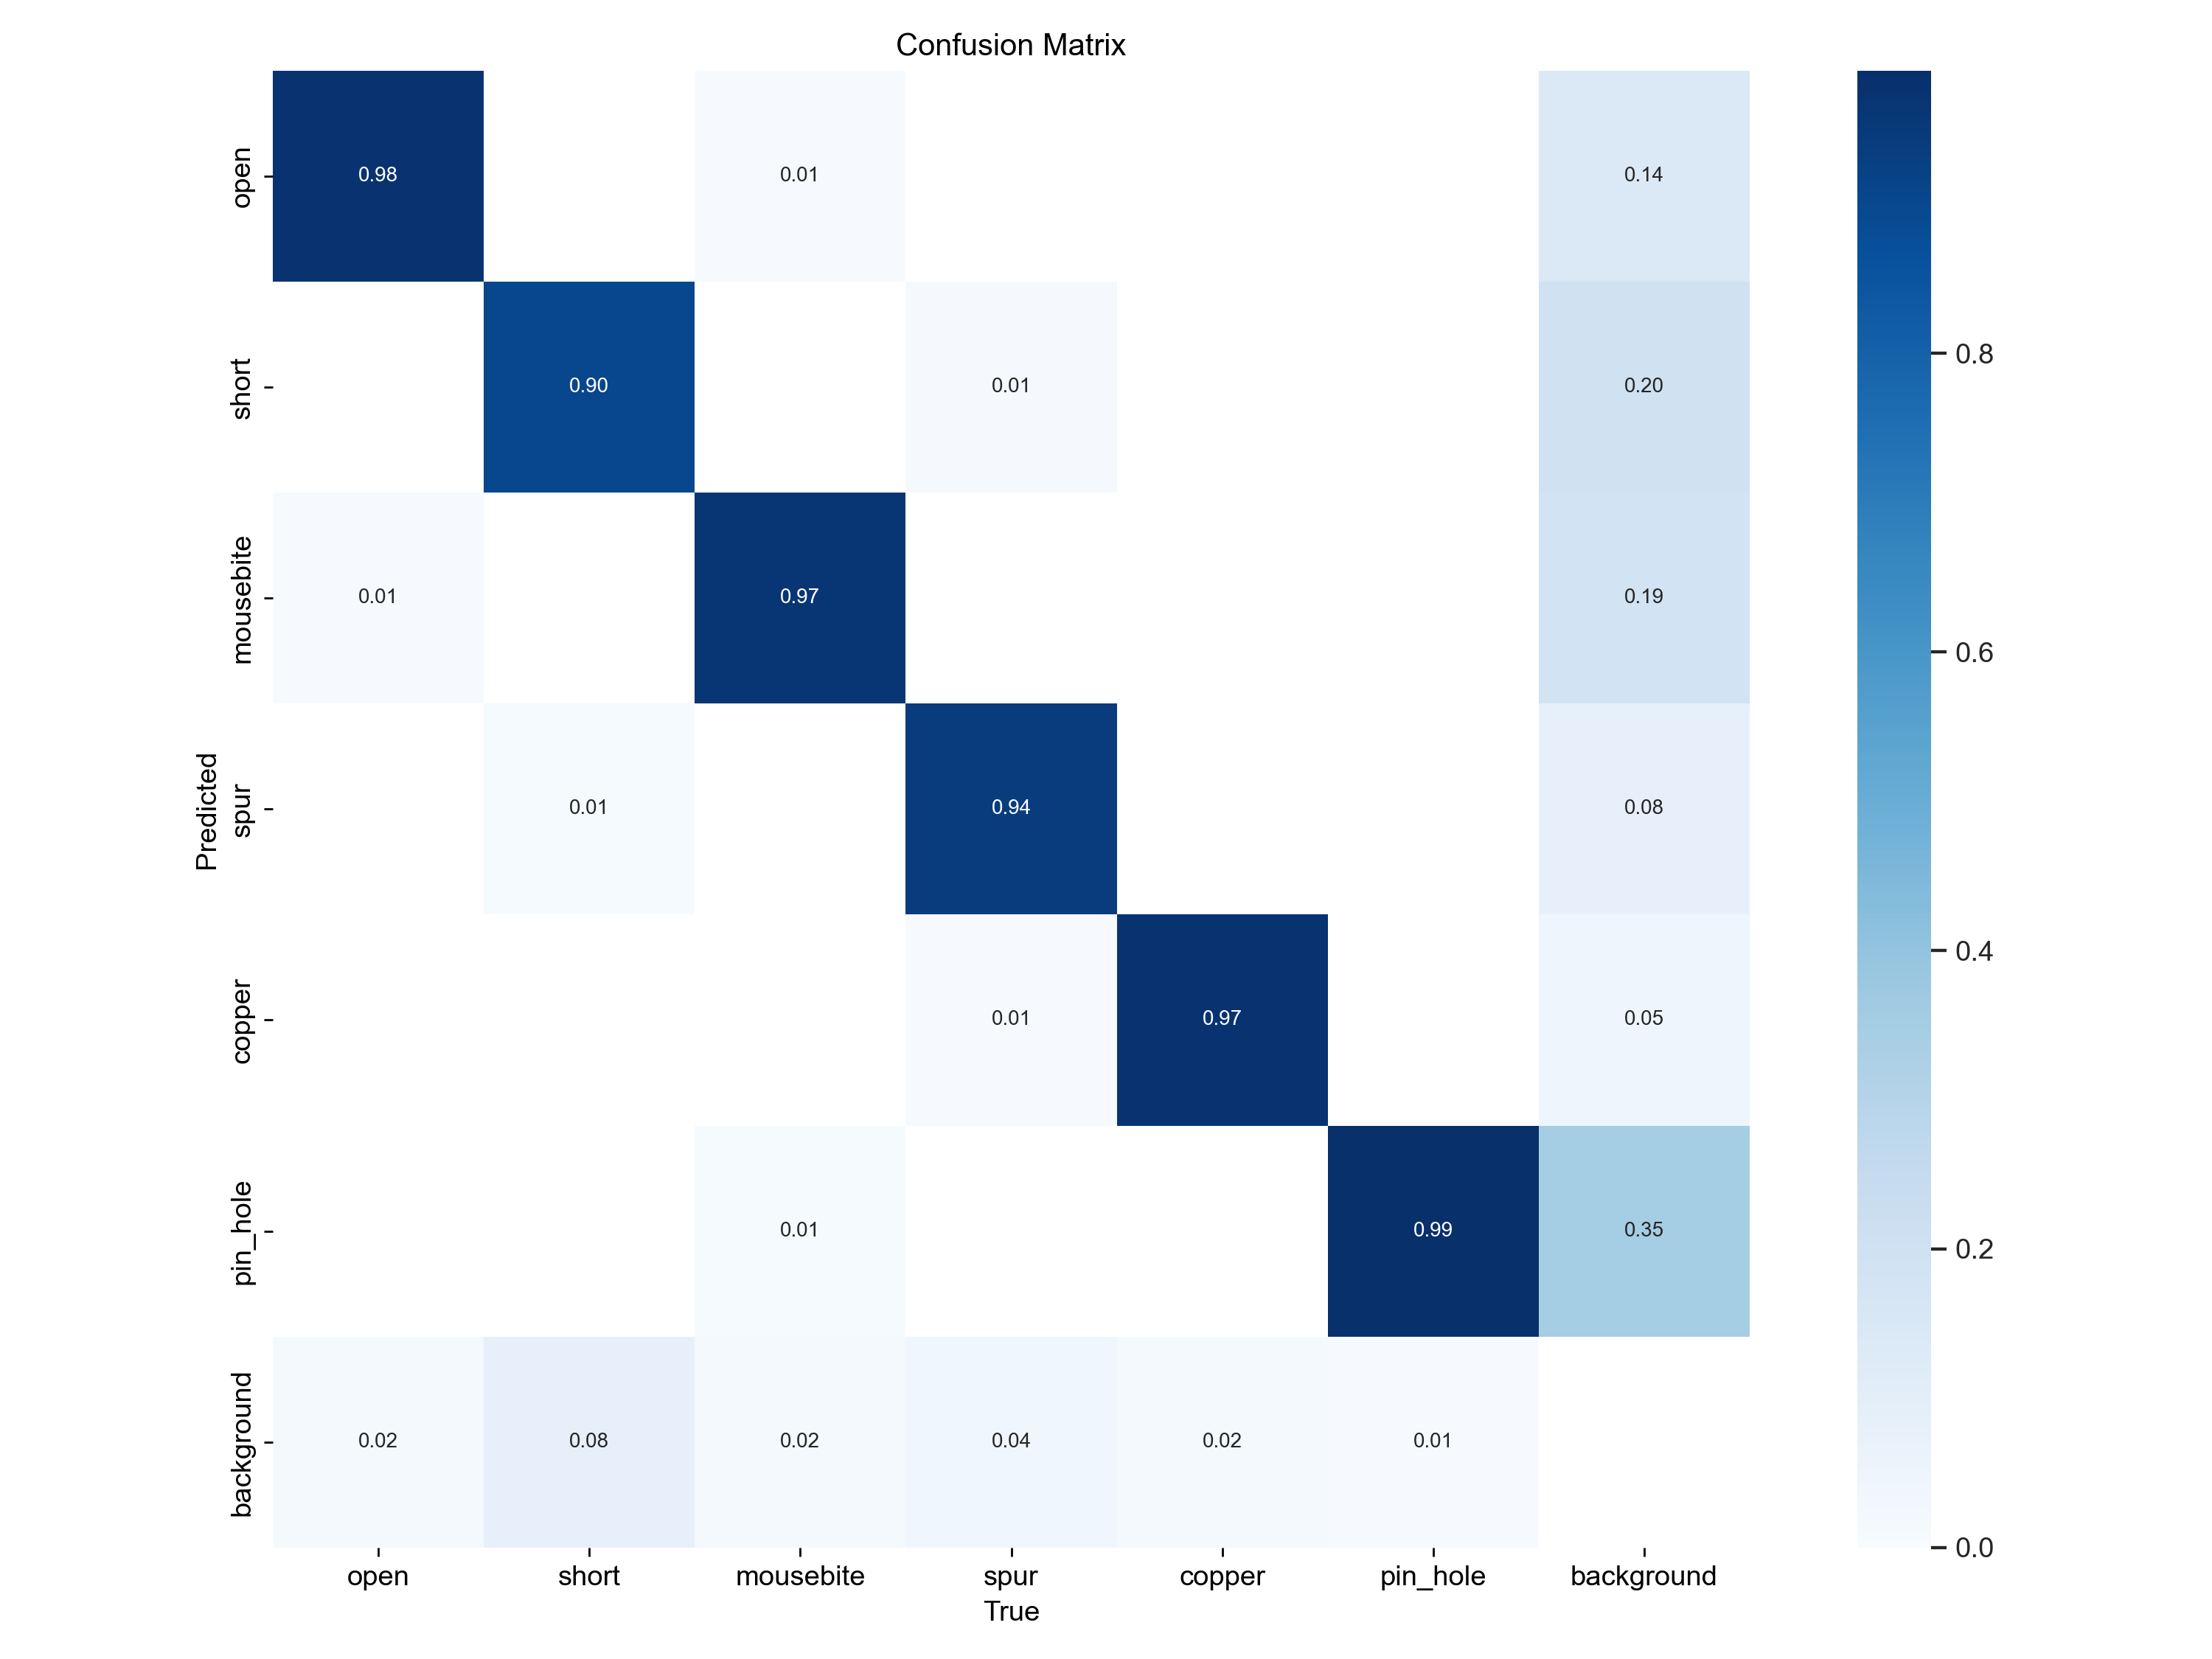
\includegraphics[width=0.98\columnwidth]{yolo_test_confusion_matrix.png}
  \caption{YOLOv5s 官方测试集混淆矩阵（含背景类行/列，可观察漏检与误检去向）。}
  \label{fig:cm}
\end{figure}

\begin{figure}[t]
  \centering
  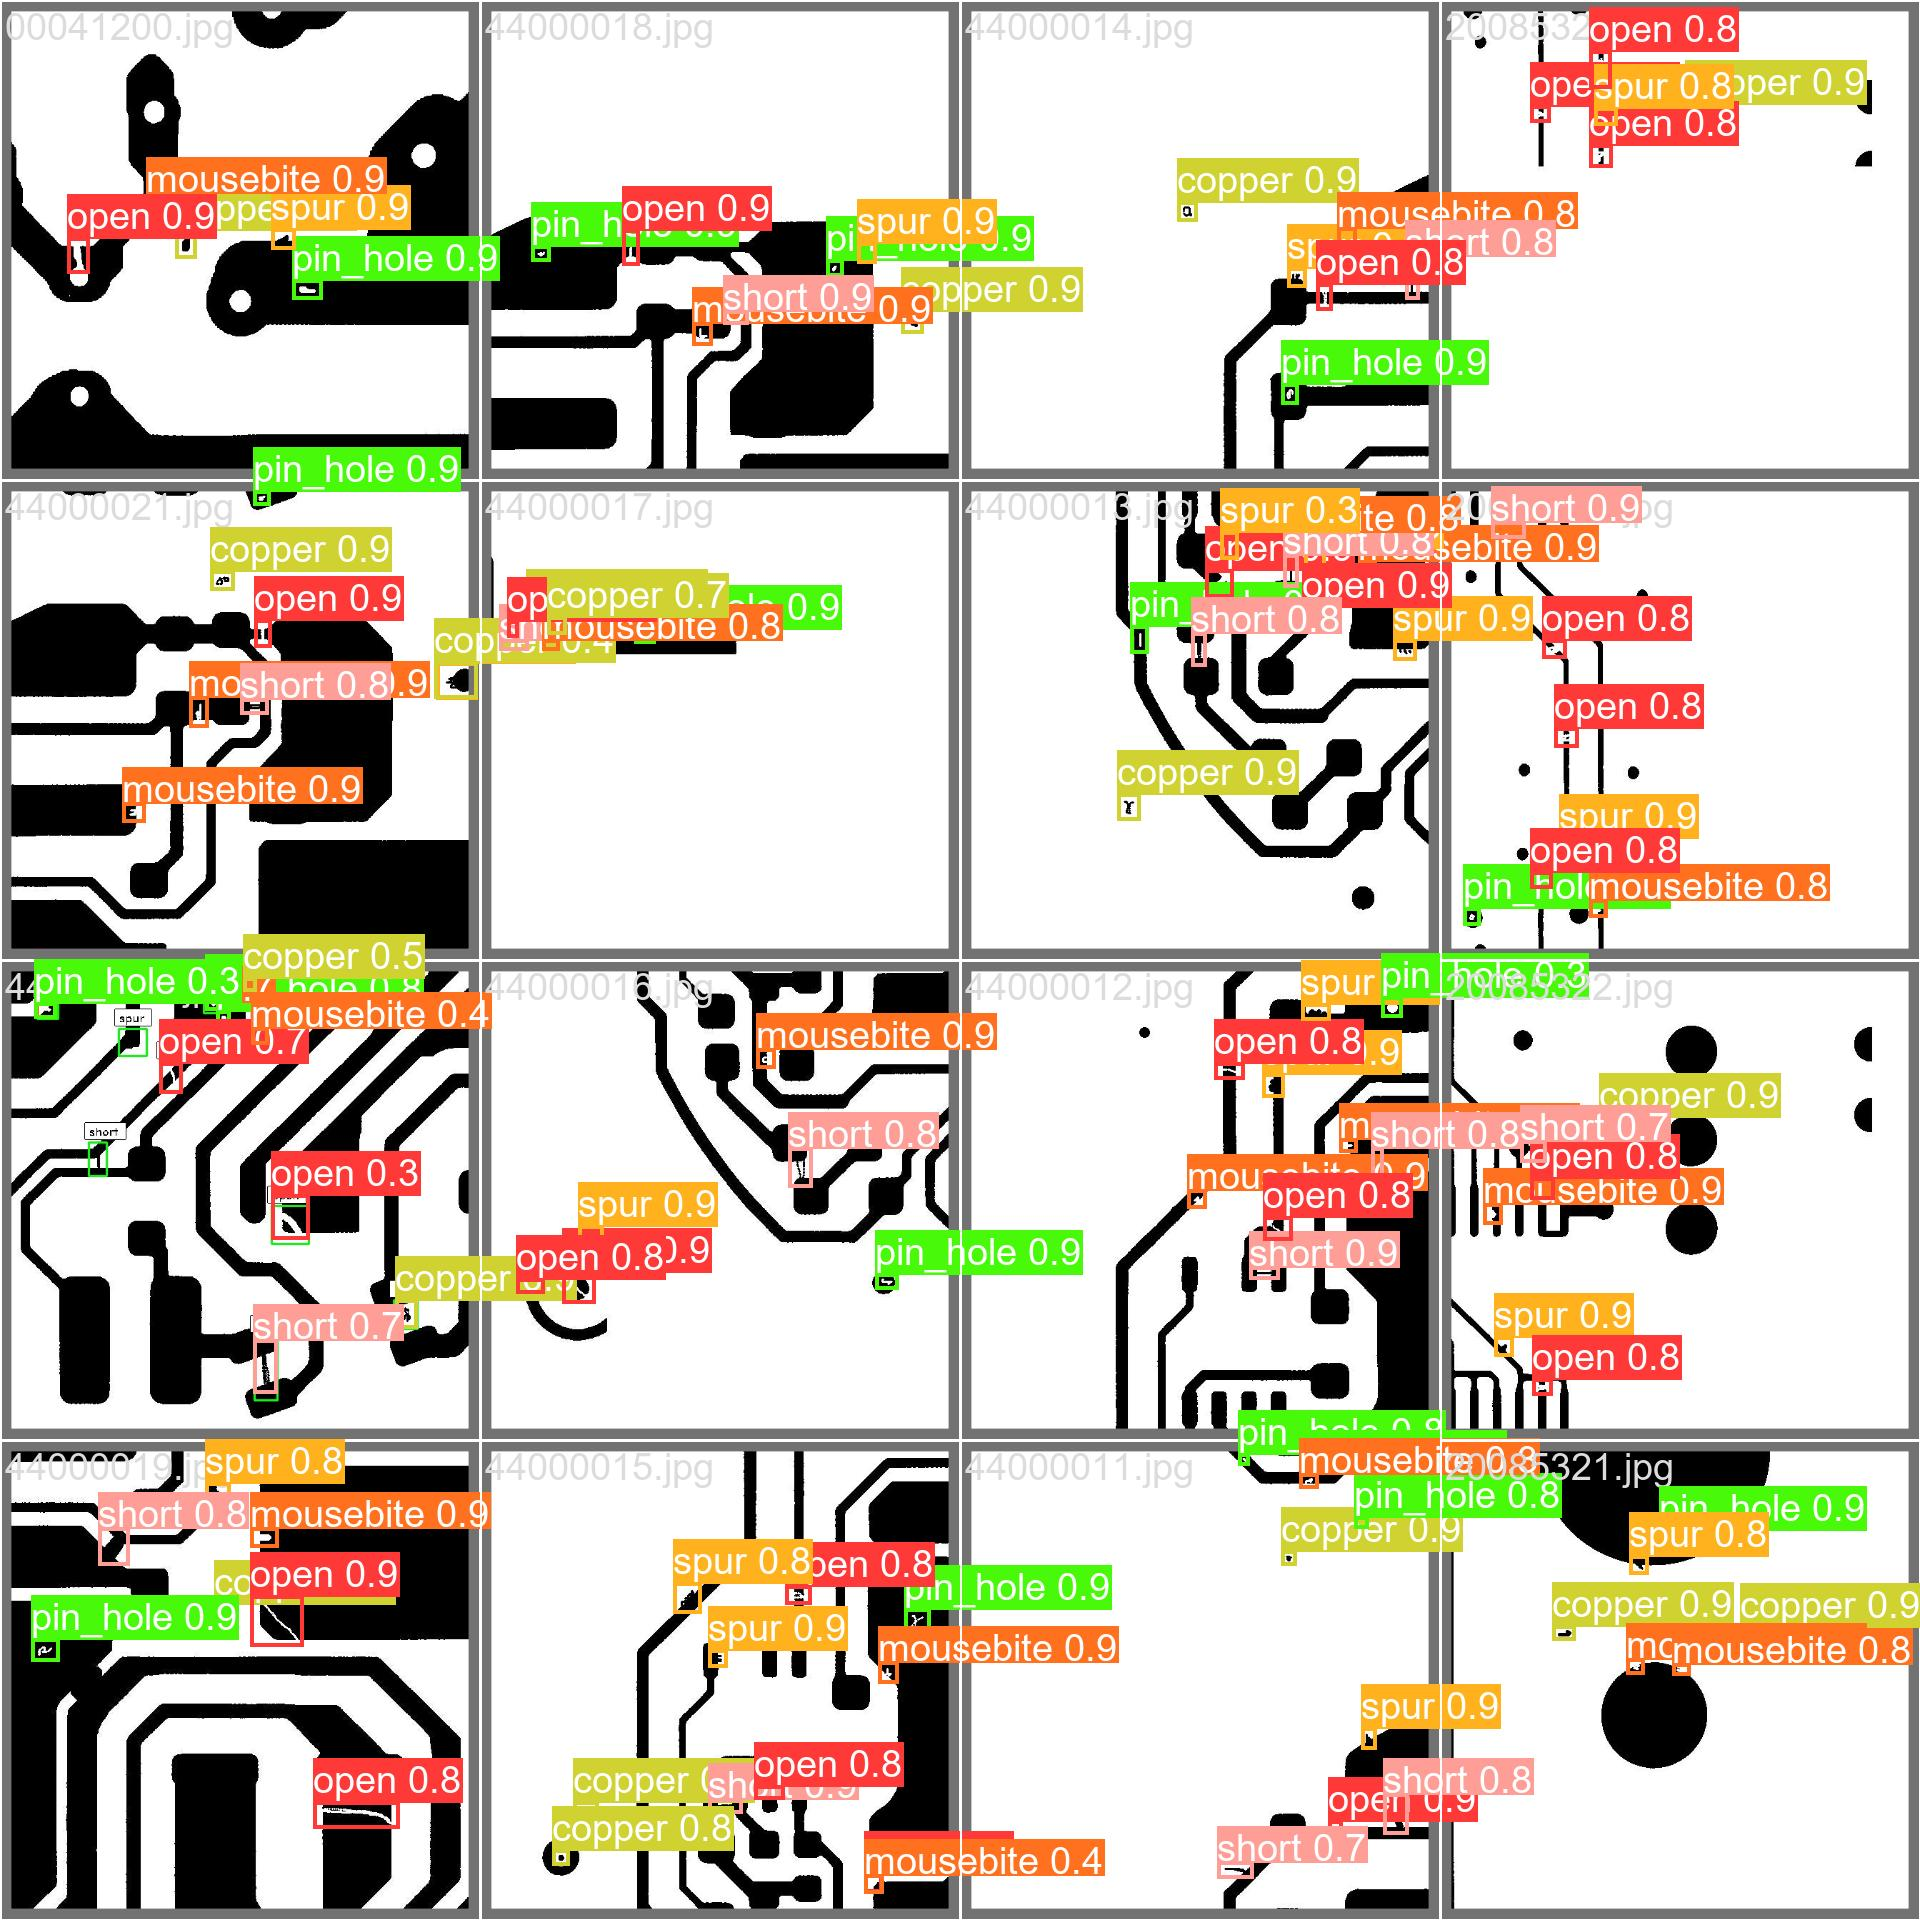
\includegraphics[width=0.98\columnwidth]{yolo_test_val_batch0_pred.jpg}
  \caption{test 预测拼图示例（val\_batch0\_pred，框上数字为置信度）。}
  \label{fig:pred}
\end{figure}

\subsection{传统图像处理基线方法结果}

表~\ref{tab:ip_metrics} 给出传统模块在官方测试集上的结果：共生成 3318 个候选框
（平均 6.636 个/图，与真值 6.28 个/图同量级），4 张图无候选；
IoU$=$0.33 下 TP 2124、FP 1194、FN 1016，P 0.640、R 0.676、F1 0.658；
IoU 提高到 0.50 时 F1 仅降至 0.648，说明匹配上的候选定位相当精确。
参数见表~\ref{tab:ip_params}，PAD 标定见表~\ref{tab:pad_sweep}。
图~\ref{fig:ipvis} 展示两个 group 的四栏流程可视化。

逐图统计显示性能高度依赖板面风格：70/500 张图 F1$=$1.0，414/500 张 F1$\ge$0.5，
逐图 F1 中位数 0.75；布局稀疏、走线较粗的 group 表现很好
（如 group92000 平均 F1 1.000、group77000 0.940、group00041 0.903），
而 FP 的约 90\%（1075/1194）集中在三个高密度细点阵 group（90100、12100、12300）。

\begin{table}[t]
\centering
\caption{传统图像处理 baseline 在官方 test 上的 box-level 指标（class-agnostic 贪心匹配；候选框共 3318 个，平均 6.636 个/图，4 张图无候选）}
\label{tab:ip_metrics}
\small
\setlength{\tabcolsep}{3pt}
\begin{tabular}{lcccccc}
\toprule
IoU 阈值 & TP & FP & FN & P & R & F1 \\
\midrule
0.33 & 2124 & 1194 & 1016 & 0.640 & 0.676 & 0.658 \\
0.50 & 2092 & 1226 & 1048 & 0.631 & 0.666 & 0.648 \\
\bottomrule
\end{tabular}
\end{table}

\begin{table}[t]
\centering
\caption{传统图像处理流水线参数（除 PAD 在 val 上标定外，其余为经验固定值）}
\label{tab:ip_params}
\small
\begin{tabular}{ll}
\toprule
参数 & 取值 \\
\midrule
中值滤波核 & $5\times 5$ \\
开运算核（椭圆） & $3\times 3$ \\
闭运算核（椭圆） & $5\times 5$ \\
连通域最小面积 & 50 px$^2$ \\
候选最小宽/高 & 8 px \\
候选最大宽/高 & 250 px \\
候选框外扩 PAD & 10 px（val 标定冻结） \\
评价 IoU 阈值 & 0.33 / 0.50 \\
候选得分 score & 连通域内平均差分强度$/255$ \\
\bottomrule
\end{tabular}
\end{table}

\begin{table}[t]
\centering
\caption{PAD 外扩量在 val 划分（100 图、674 框）上的标定结果（F1）}
\label{tab:pad_sweep}
\begin{tabular}{ccc}
\toprule
PAD (px) & F1@IoU=0.33 & F1@IoU=0.50 \\
\midrule
0 & 0.062 & 0.006 \\
4 & 0.557 & 0.134 \\
6 & 0.691 & 0.498 \\
8 & 0.700 & 0.666 \\
\textbf{10} & \textbf{0.703} & \textbf{0.688} \\
12 & 0.700 & 0.686 \\
14 & 0.700 & 0.682 \\
16 & 0.697 & 0.632 \\
\bottomrule
\end{tabular}
\end{table}


\begin{figure*}[tp]
  \centering
  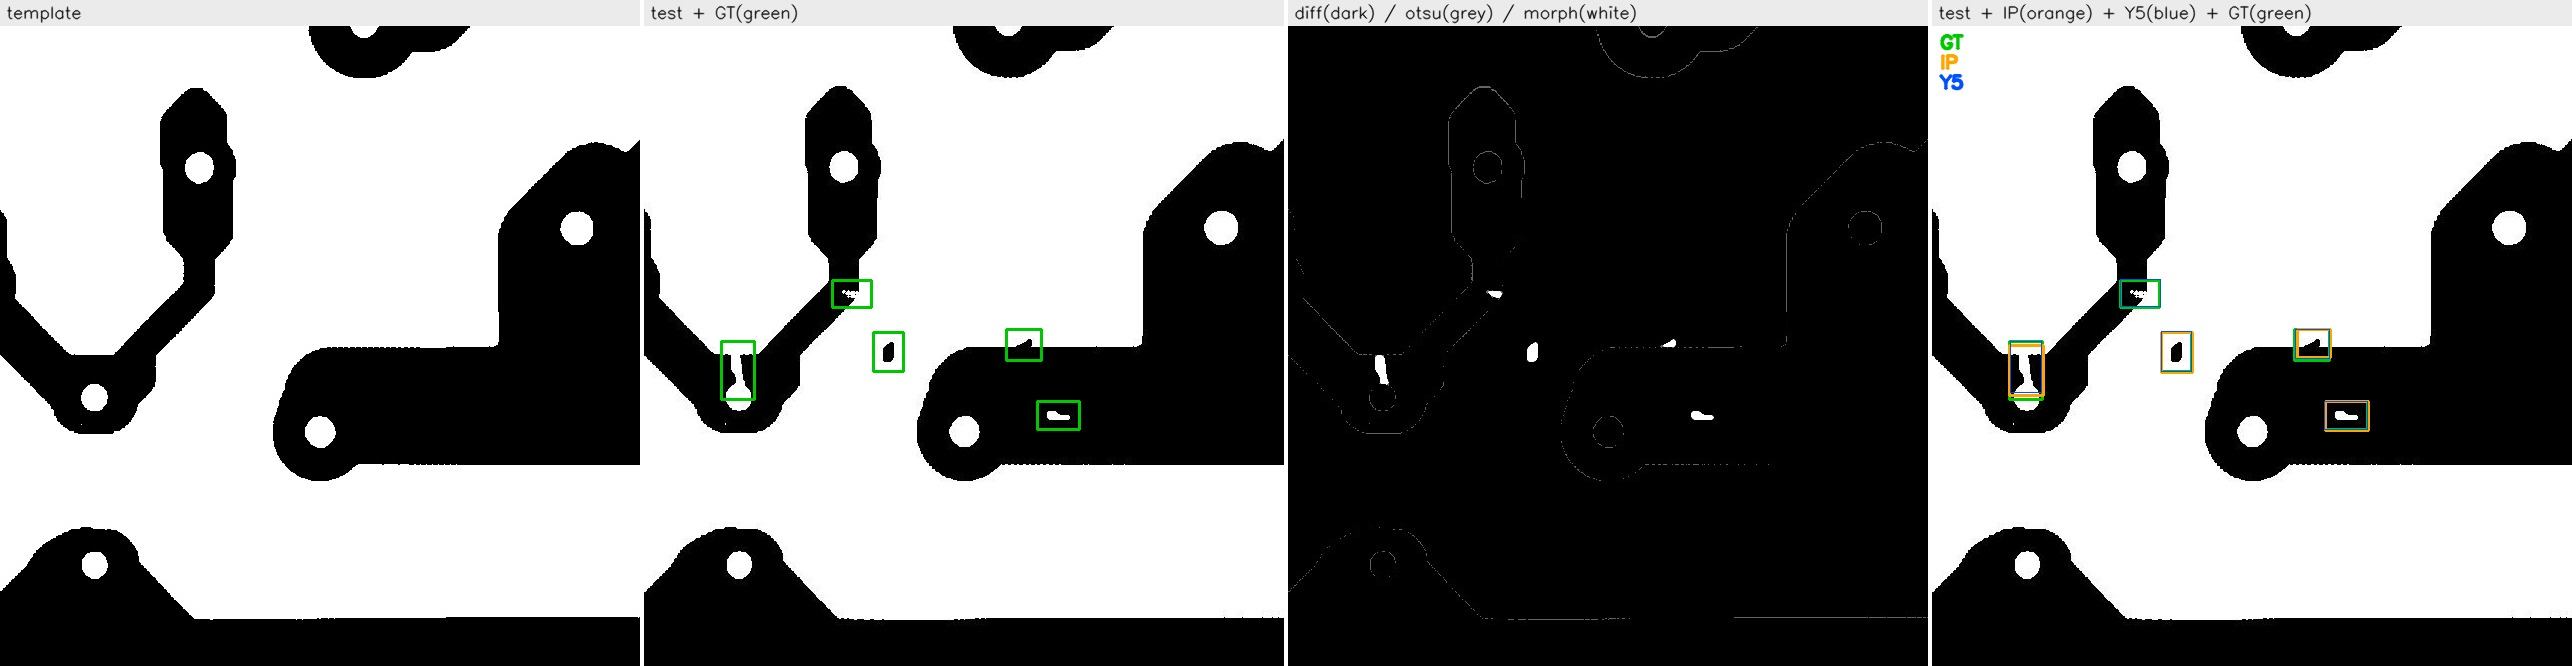
\includegraphics[width=0.92\textwidth]{ip_vis_00041200.jpg}\\[2pt]
  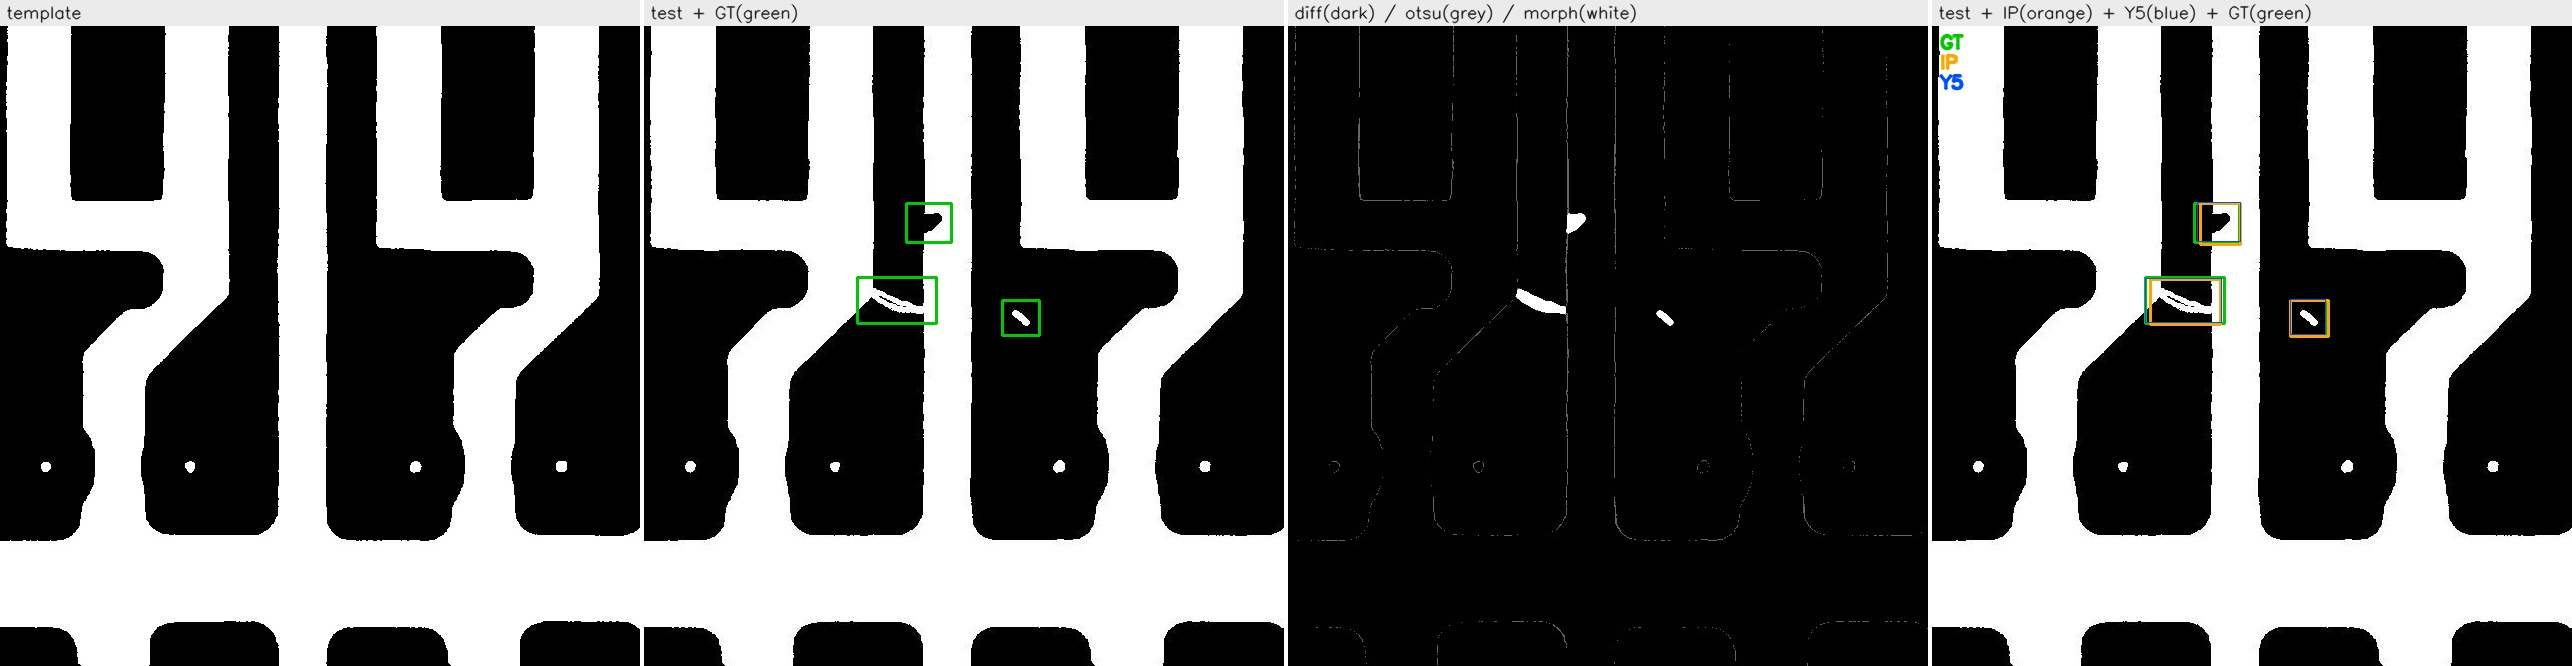
\includegraphics[width=0.92\textwidth]{ip_vis_92000111.jpg}
  \caption{传统流水线四栏可视化两例（上：group00041；下：group92000）。
  自左至右：模板图；待测图$+$真值框（绿）；差分/Otsu/形态学复合诊断图
  （暗底为差分，灰为 Otsu 保留但被形态学去除，白为最终掩码）；
  待测图$+$传统候选（橙）$+$YOLO 预测（蓝，conf$\ge$0.25）$+$真值（绿）。}
  \label{fig:ipvis}
\end{figure*}

\subsection{错误分析与互补性讨论}

\textbf{YOLOv5s 的误差结构。}mAP50（0.968）与 mAP50:95（0.594）的差距表明模型的
粗定位很强、高 IoU 精细定位仍有限，这与缺陷本身边界模糊、真值框带标注边距有关。
分类别看，short 相对薄弱：其召回 0.863 为六类最低，直观原因是短路常表现为
细窄的桥接导体，外观与正常走线相似；pin\_hole 则查全高（0.979）但查准较低（0.865），
存在把铜面上正常孔洞误报为针孔的倾向，混淆矩阵（图~\ref{fig:cm}）中相应的
背景类误检可以佐证。

\textbf{传统方法的 FP/FN 机理。}FP 集中来源于配准残差：高密度细点阵板面上
1--2\,px 的对齐误差会在几乎所有结构边缘产生差分晕环，开运算无法完全去除，
存活为大量中等尺寸的噪声连通域（图~\ref{fig:fail}a）；FN 则集中于弱差分信号的
细小缺陷——为压制噪声而设的面积/宽高过滤门槛会一并滤除这些小连通域，
4 张零候选图即属此类（图~\ref{fig:fail}b、c）。这体现了固定阈值流水线在
精度与召回之间的固有张力。

\textbf{互补性。}两类方法的失败模式并不重合：4 张传统方法零候选的图上
YOLOv5s 六类全部检出（图~\ref{fig:fail}c）；反过来，传统方法也在 43 张图上
找回了共 49 个 YOLOv5s（conf$\ge$0.25）漏检的真值框（图~\ref{fig:fail}d）。
这说明基于模板先验的差分证据与基于学习的外观证据是两种不同的信息来源，
传统模块可以作为候选区域生成与可解释诊断工具（其差分/阈值/形态学中间结果全程可视）
辅助检测主线，而不是替代它。

\begin{figure*}[!t]
  \centering
  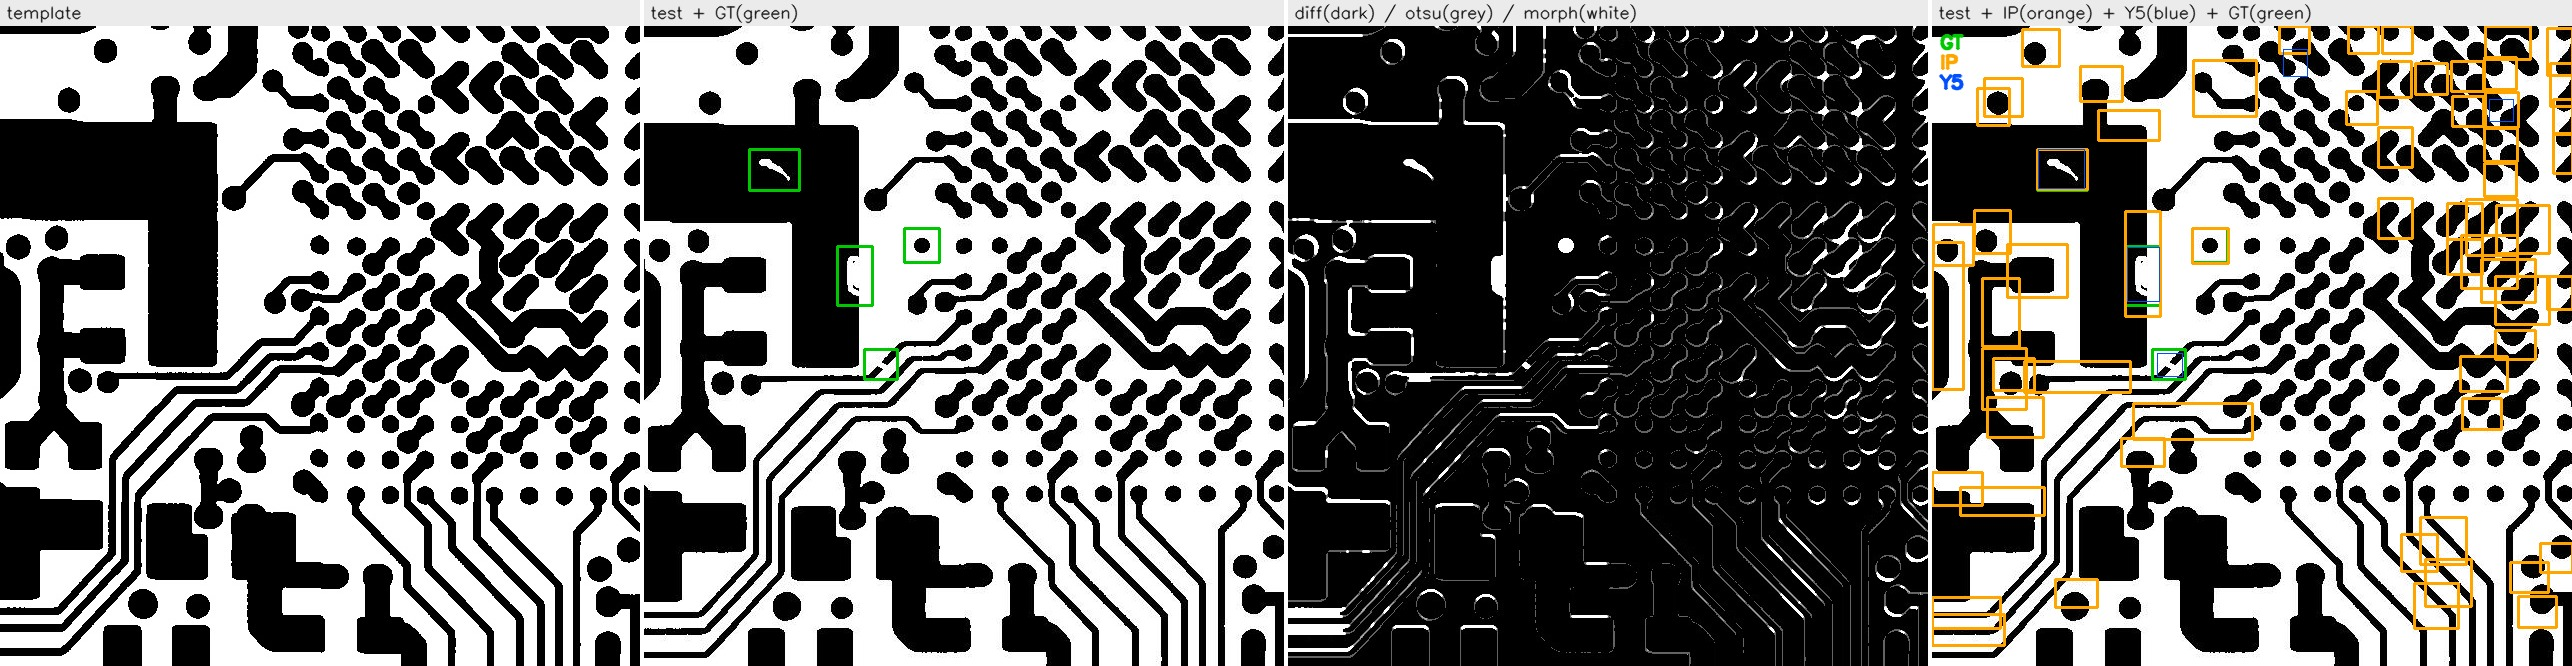
\includegraphics[width=0.88\textwidth]{fail_fp_90100028.jpg}\\[1pt]
  {\footnotesize (a) FP 密集案例：配准残差导致大量候选}\\[2pt]
  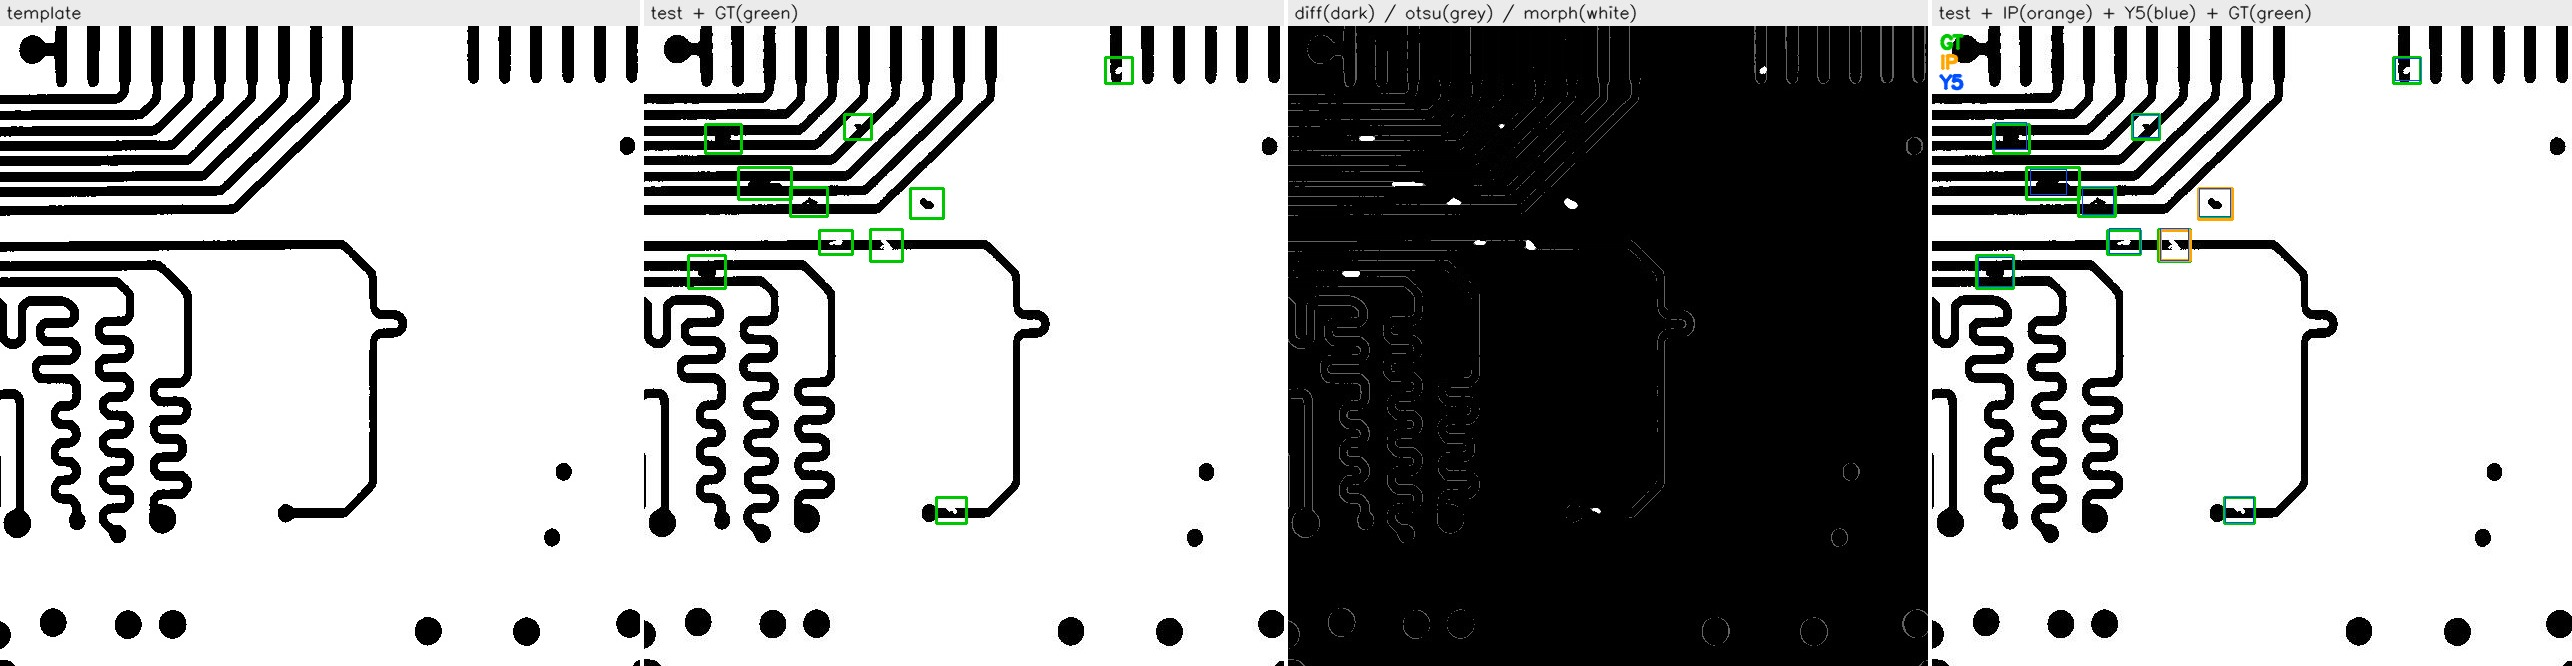
\includegraphics[width=0.88\textwidth]{fail_fn_20085310.jpg}\\[1pt]
  {\footnotesize (b) FN 密集案例：弱差分小缺陷被过滤}\\[2pt]
  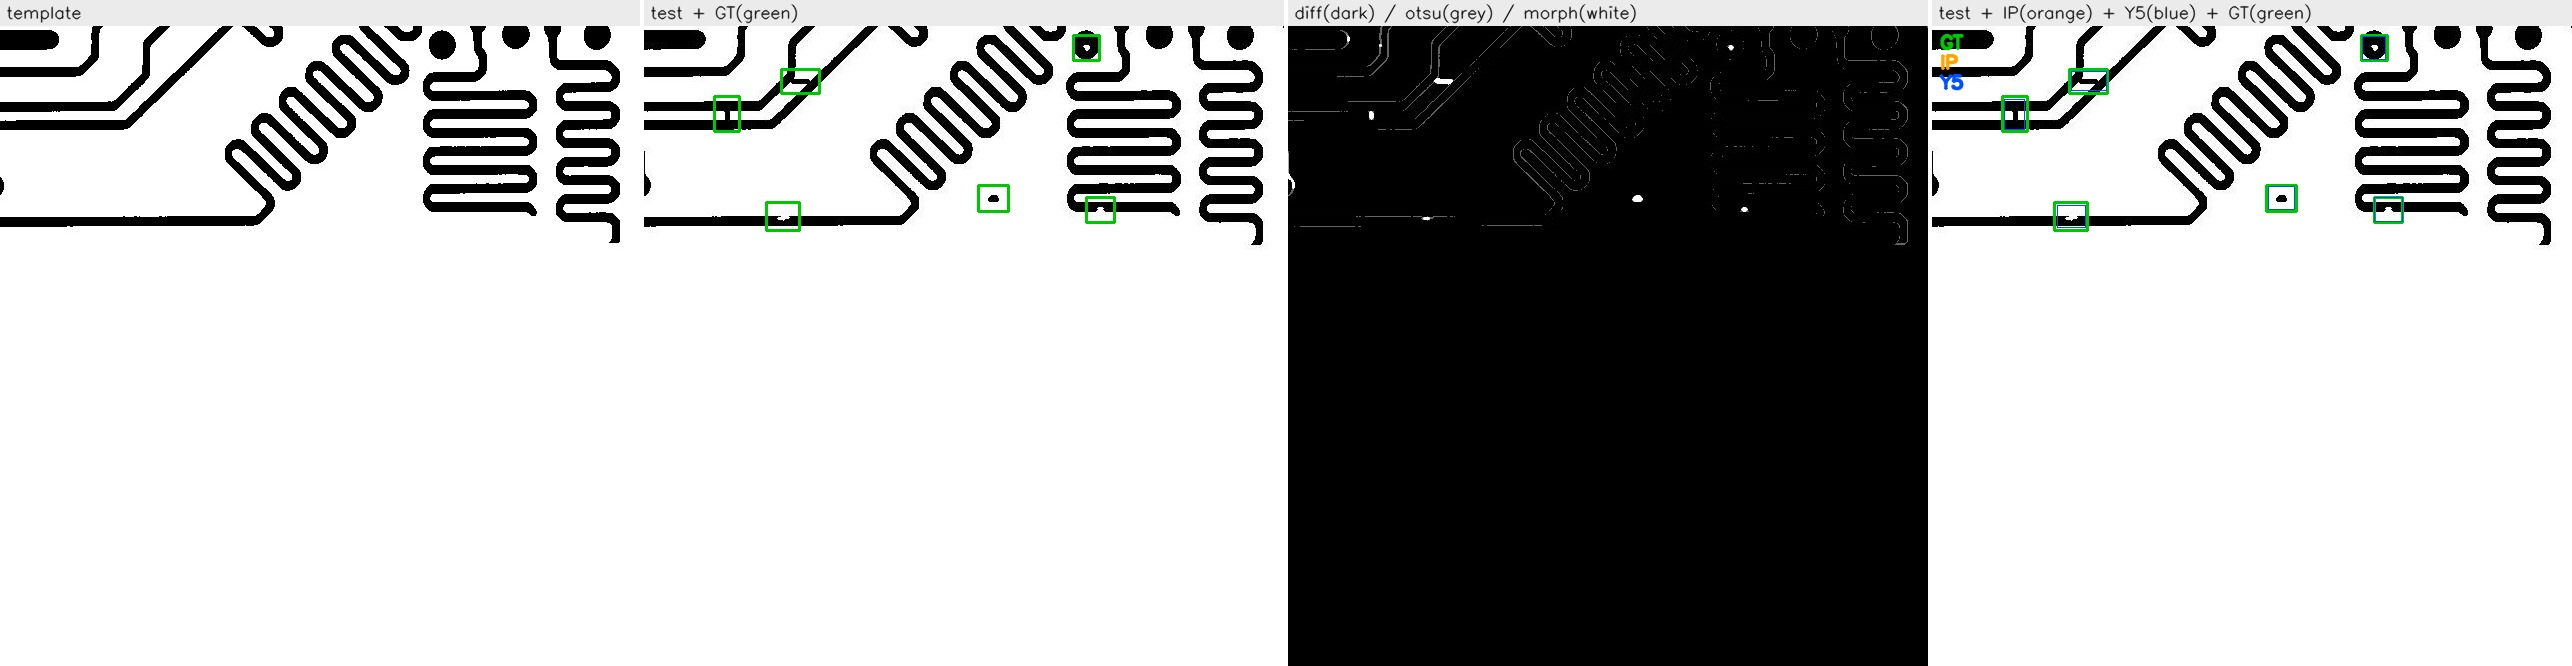
\includegraphics[width=0.88\textwidth]{fail_yolo_ok_ip_fail_20085298.jpg}\\[1pt]
  {\footnotesize (c) YOLO 检出而传统方法零候选}\\[2pt]
  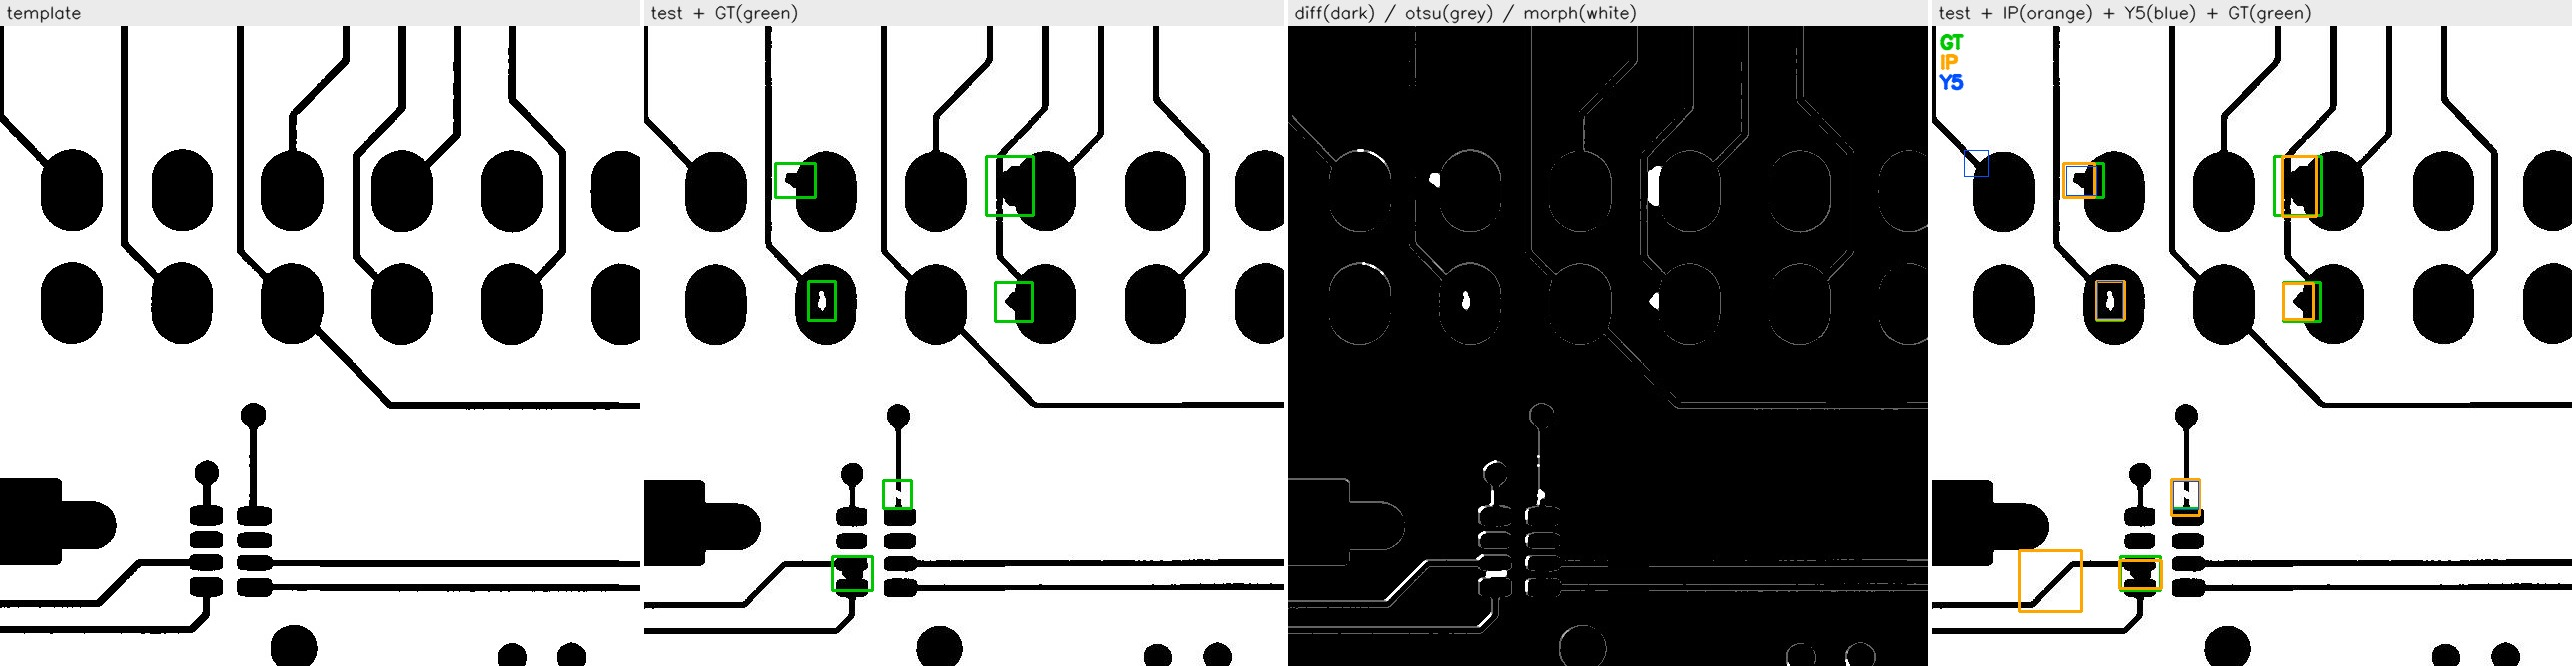
\includegraphics[width=0.88\textwidth]{fail_ip_found_yolo_miss_90100033.jpg}\\[1pt]
  {\footnotesize (d) 传统方法补充定位 YOLO 漏检框}
  \caption{四类代表性失败/互补案例，栏序同图~\ref{fig:ipvis}。}
  \label{fig:fail}
\end{figure*}

\clearpage
\raggedbottom
\section{局限性}\label{sec:limits}

评价协议方面，传统方法是类别无关的候选方法，不输出六类类别；YOLOv5s 的 mAP 与传统方法的
F1 分别基于类别相关 PR 积分和类别无关贪心匹配，不能直接作数值比较，本文只在定位与可视化
层面讨论二者差异。

传统方法方面，外扩边距 PAD 用于缓解连通域外接框与标注框尺度约定不一致的问题，具体数值在
验证集上标定并固定；其余滤波核、形态学核、面积与宽高门限均为经验固定值。该方法对
配准残差、密集纹理以及弱差分的小缺陷较为敏感。

模型与数据外推方面，mAP50 明显高于 mAP50:95，高 IoU 精细定位能力仍有限；short 是相对困难类别
（R 0.863、mAP50:95 0.482），pin\_hole 查全较高但 precision 较低（0.865），存在误报倾向。
测试集中 66.4\% 的图像来自未见 group，这一结果仅反映 group 级差异下的表现；DeepPCB 图像经
二值化预处理，当前结果不能直接外推到真实工业部署。

\section{总结}\label{sec:concl}

本文在 DeepPCB 上完成了从数据核查、格式转换、脚本化自检，到 YOLOv5s 训练与官方测试集
评估，再到传统图像处理候选生成模块的完整课程实践。YOLOv5s 在官方测试集上取得
P 0.951 / R 0.944 / mAP50 0.968 / mAP50:95 0.594；传统"差分$+$Otsu$+$形态学$+$连通域"
模块作为类别无关基线方法取得 IoU$=$0.33 下 F1 0.658，并提供了可解释的中间结果
与失败案例分析。两类方法在本数据集上的失败模式有所不同，说明模板差分证据与学习式外观特征
具有一定互补性。
后续可进一步尝试将传统候选用于辅助后处理，并在更接近原始工业图像的场景中验证。

\section*{代码与材料说明}

本项目的报告、代码、主要运行日志、结果表格和可视化图已随课程材料整理提交。完整 DeepPCB
图片数据不随报告打包，可从官方仓库获取。代码与材料仓库：
\url{https://github.com/bronlemesja32-zzz/deeppcb-yolov5-dip-project}。

\phantomsection\label{page:refs}
\printbibliography[title={参考文献}]

\end{document}
